% 
% topic Template for ME3050 -  Dynamics Modeling and Controls - Tennessee Technological University
%
% Spring 2020 - Summer 2020
% Tristan Hill, May 07, 2020
% Dyanmics Review - Topic 1 - What is System Dynamics?
%

\documentclass{beamer}                         % for presentation (has nav buttons at bottom)
%\documentclass[handout]{beamer}  % for handout 
\usepackage{beamerthemesplit}
\usepackage{amsmath}
\usepackage{listings}
\usepackage{multicol}

\beamertemplateballitem

\definecolor{TTUpurple}{rgb}{0.3098, 0.1607, 0.5176} % TTU Purple (primary)
\definecolor{TTUgold}{rgb}{1.0000, 0.8666, 0.0000} % TTU Gold (primary)

\setbeamercolor{palette primary}{bg=TTUpurple,fg=TTUgold}
\setbeamercolor{palette secondary}{bg=black,fg=TTUgold}
\setbeamercolor{palette tertiary}{bg=black,fg=TTUpurple}
\setbeamercolor{palette quaternary}{bg=TTUgold,fg=black}
\setbeamercolor{structure}{fg=TTUpurple} % itemize, enumerate, etc
\setbeamercolor{section in toc}{fg=TTUpurple} % TOC sections

%\usefonttheme{professionalfonts}

\newcommand{\TNUM}{1\hspace{2mm}} % topic Number 

\newcommand{\Lagr}{\mathcal{L}} % lagrangian

\newcommand{\vspccc}{\vspace{6mm}\\} % large vertical space
\newcommand{\vspcc}{\vspace{4mm}\\}   % medium vertical space
\newcommand{\vspc}{\vspace{2mm}\\}     % small vertical space

\newcommand{\hspcccc}{\hspace{10mm}} % large horizontal space
\newcommand{\hspccc}{\hspace{6mm}} % large horizontal space
\newcommand{\hspcc}{\hspace{4mm}}   % medium horizontal space
\newcommand{\hspc}{\hspace{2mm}}     % small horizontal space


\author{ME3050 - Dynamics Modeling and Controls} % original formatting from Mike Renfro, September 21, 2004


\newcommand{\firsttitle}{Dynamics Review - Topic \TNUM}
\newcommand{\secondtitle}{What is System Dynamics?}% second line of the title of this presentation , aka the topic of this topic

\title{\firsttitle}

\date{May 27, 2020}

\begin{document}

\lstset{language=MATLAB,basicstyle=\ttfamily\small,showstringspaces=false}

% Section 0: Outline
\frame{\titlepage \center\textbf{\secondtitle}\vspace{5mm}\\}

\frame{

\large \textbf{Topic \TNUM - \secondtitle} \vspace{3mm}\\

%Topics : \vspace{3mm}\\ % ' topics' are beamer 'sections' - TWH

\begin{itemize}
	\item Welcome Back!\vspace{3mm}\\ % Section 1
	\item Definition of {\it Dynamics}\vspace{3mm}\\% Section 2
	\item Modeling and Analysis \vspace{3mm}\\ %Section 3
	\item Model Based Design\vspace{3mm}\\ % Section 4
	%\item Example\vspace{3mm}\\ % Section 5 - 5 is almost too many...
\end{itemize}
}

% Section 1
\section{Welcome Back!}

\frame{
\frametitle{Welcome to New Video topics}
\large{\it Welcome Back!\vspace{3mm}\\}

\begin{itemize}
\item Things are going to be different but we will still learn! \vspace{3mm}\\
\item These new outlines should help keep me/us on track.  \vspace{3mm}\\
\item The material will be organized in 10-15 min videos, and you can watch them at anytime. \vspace{3mm}\\
\end{itemize}

}

% Section 2
\section{Definition of Dynamics}

\frame{
\frametitle{Definition of Dynamics}

\large
Dynamics is ...\vspcc

the study of how moving objects behave, \vspcc
or \vspcc
an area of mechanics that studies movement and its causes,\vspcc
or \vspcc
%\Large{"The dynamical system concept is a mathematical formalization for any fixed "rule" which describes the time dependence of a point's position in its ambient space. "} \vspace{5mm} \\

{\it system dynamics} is the study of {\bf modeling} and {\bf analysis} of dynamical systems as a function of time.\vspc

}

% Section 3
\section{Modeling and Analysis}

\frame{
\frametitle{What is Mathematical Modeling?}

A mathematical model is a description of a system using mathematical concepts and language. The process of developing a mathematical model is termed mathematical {\bf modeling} ... \vspc
...  are used in the natural sciences and engineering disciplines ...  \href{https://en.wikipedia.org/wiki/Mathematical_model}{\tiny Wikipedia}

\begin{itemize}
\item Model Simplification
\item Force and Loading Analysis with FBDs
\item Fundamental Laws Lead to Equations of Motion
\item Newton's Second Law and Conservation of Energy

\end{itemize}

}

\frame{
\frametitle{What is Analysis?}

{\bf Analysis} is the process of breaking a complex topic or substance into smaller parts in order to gain a better understanding of it... \href{https://en.wikipedia.org/wiki/Analysis}{\tiny Wikipedia}

\begin{itemize}
\item Model Simplification
\item Force and Loading Analysis with FBDs
\item Fundamental Laws Lead to Equations of Motion
\item Newton's Second Law and Conservation of Energy

\end{itemize}

}

% Section 4
\section{Model Based Design}

\frame{
\frametitle{Model Based Design}

Model-Based Design (MBD) is a mathematical and visual method of addressing problems associated with designing complex control, signal processing and communication systems. It is used in many motion control, industrial equipment, aerospace, and automotive applications... \href{https://en.wikipedia.org/wiki/Model-based_design}{\tiny Wikipedia}


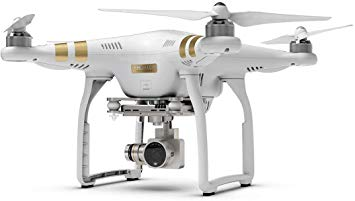
\includegraphics[scale=.25]{dji_phantom.jpg}\hspccc
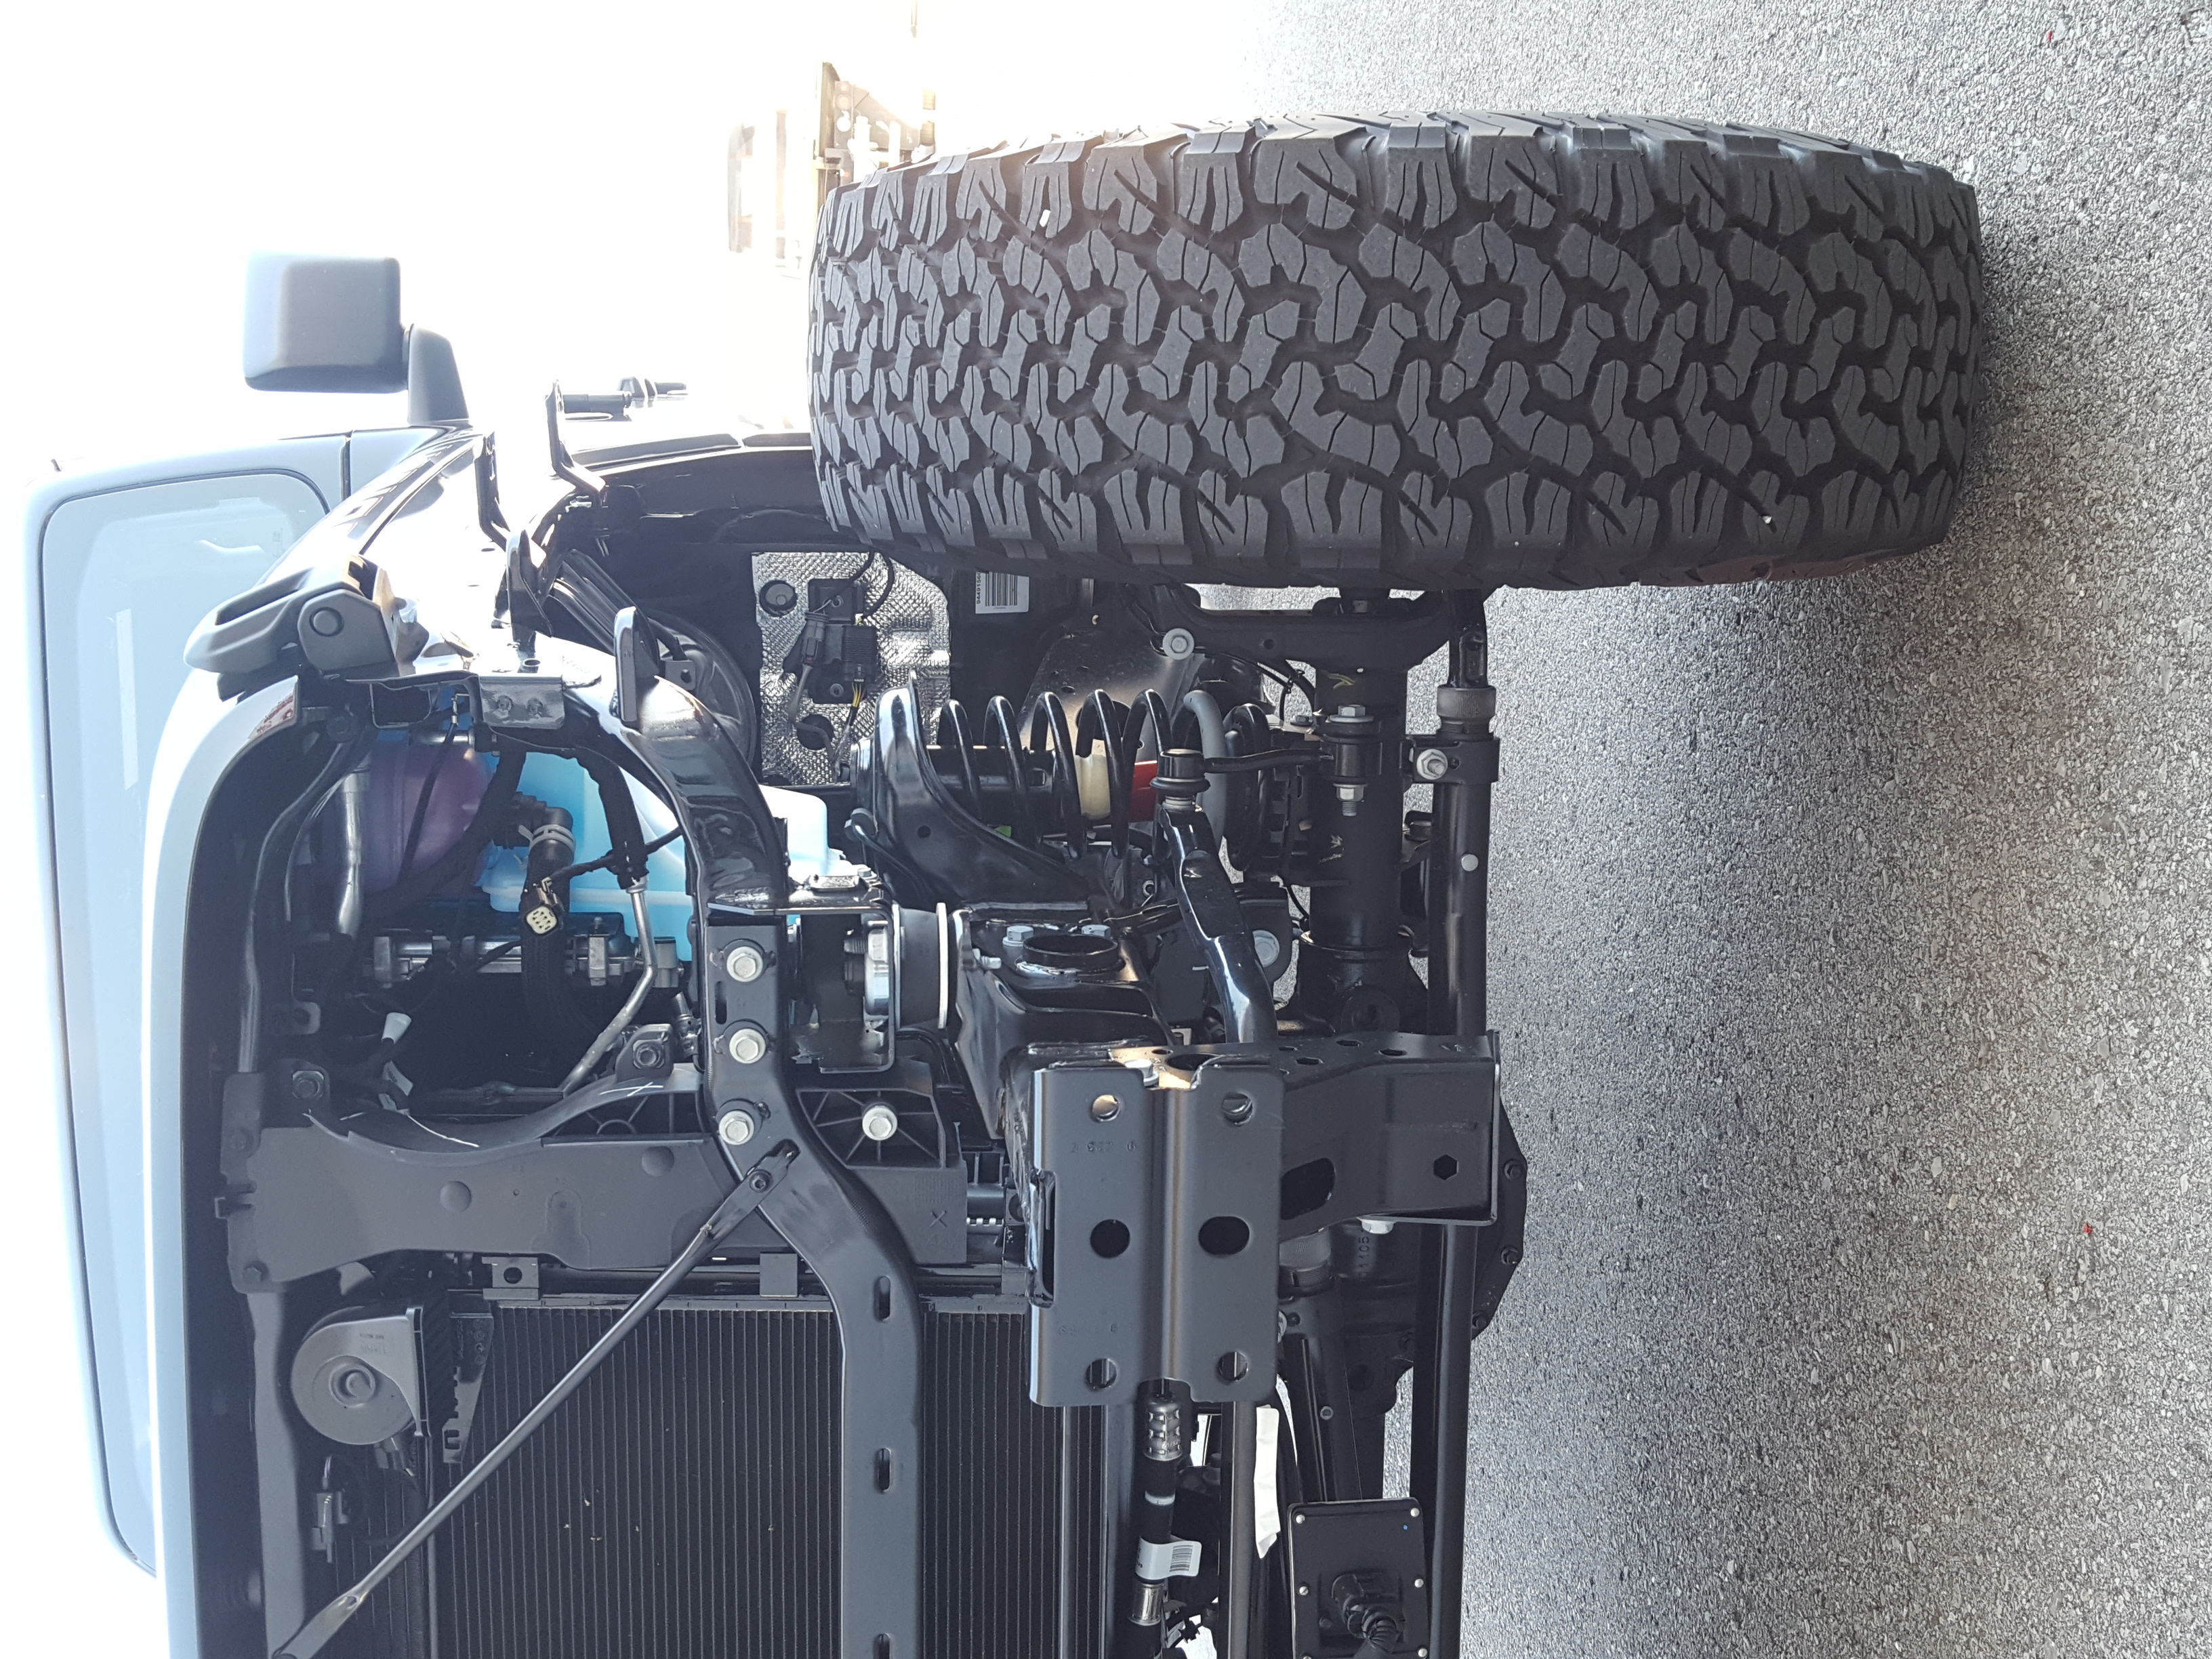
\includegraphics[scale=.025,angle=-90,origin=c]{jeep_01.jpg} \hspccc
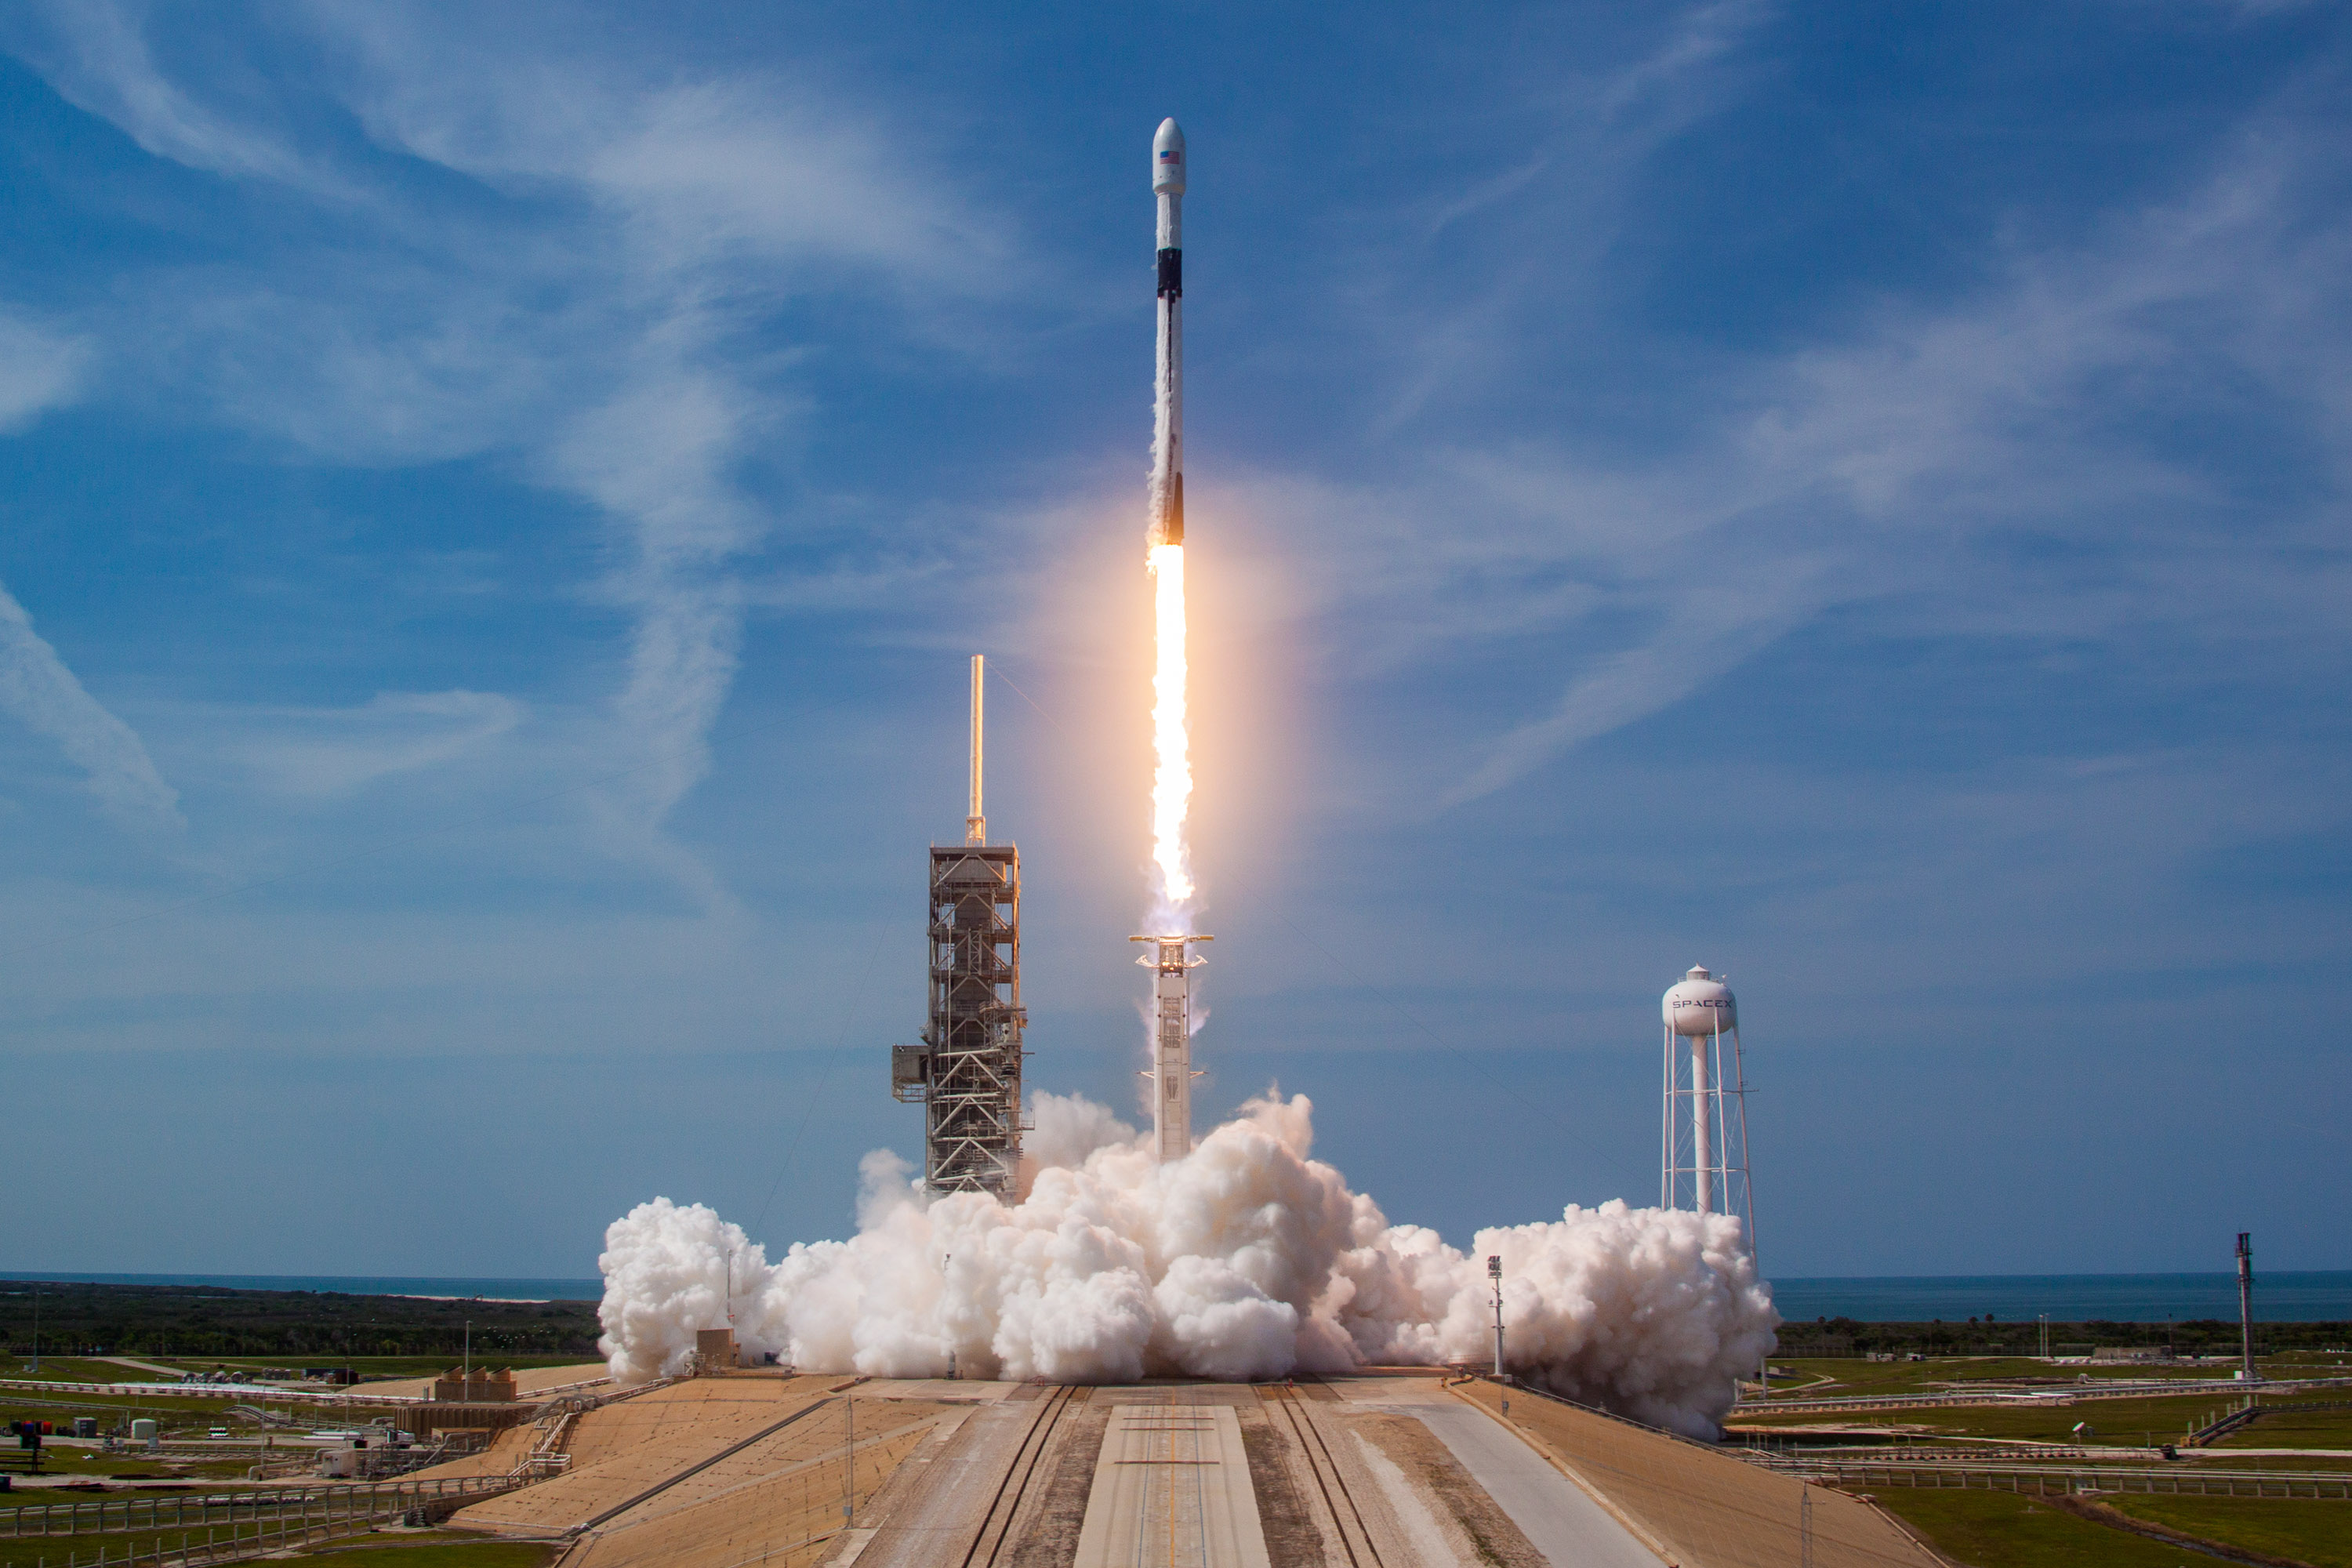
\includegraphics[scale=.15]{falcon9.jpg} \\

}



\end{document}
%	\item \textbf{ \LARGE \B Dynamic\K} \\
%			
%			\Large{"Dynamics is the study of how moving objects behave. Dynamics is the part of mechanics that studies movement and its causes. The study of the causes of motion and changes in motion is known as dynamics. Dynamics is the study of how moving objects behave."} \vspace{5mm} \\
%
%			\Large{"The dynamical system concept is a mathematical formalization for any fixed "rule" which describes the time dependence of a point's position in its ambient space. "} \vspace{5mm} \\
%
%	\item \textbf{ \Large Translational Motion } 
%\begin{itemize}
%\item Position
%\item Velocity 
%\item Acceleration \vspace{2mm}\\
%\end{itemize} 
%
%	\item \textbf{ \Large Rotational Motion }
%\begin{itemize}
%\item Position
%\item Velocity 
%\item Acceleration \vspace{2mm}\\
%\end{itemize} 		
%	
%	\item \textbf{ \Large Particle Motion } 
%\begin{itemize}
%\item What do mean by this? \vspace{2mm}\\
%\end{itemize}
%\item \textbf{ \Large Rigid-Body Motion } 
%\begin{itemize}
%\item What do mean by this specifically? Mathematically?
%\end{itemize}
%
%\newpage
%\item \textbf{ \Large Degrees of Freedom (DOF) } 
%	\begin{itemize}
%\item What does this mean? \vspace{25mm}\\
%\item Examples:
%\end{itemize}
%
%\newpage
%	\item \textbf{ \Large The \B dynamics \K are represented as ordinary \vspace{3mm}\\
%differential equations called the \\\\ \underline{\hspace{60mm}} of \underline{\hspace{60mm}}.} \vspace{2mm}\\
%
%	\item \textbf{ \Large Deriving the 	\underline{\hspace{60mm}} of \underline{\hspace{60mm}} \vspace{1mm}\\is typically done in one of two ways.} \\
%	\begin{enumerate}
%		\item Newtonian Approach - Vector Based Method \vspace{3mm}\\
%		\begin{itemize}
%\item Translational\\
%\item Rotational  \vspace{10mm}\\
%\end{itemize} 
%\item Conservation of Energy Approach - Energy Based Method \vspace{3mm}\\
%		\begin{itemize}
%\item Kinetic Energy\\
%\item Potential Energy\\  
%\end{itemize} 
%	\end{enumerate}
%
%\newpage
%
%\item \textbf{ \Large  Example:} DJI Phantom with 3-axis Camera Gimbal \\
%
%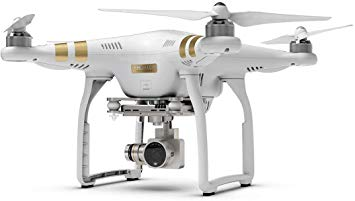
\includegraphics[scale=1]{dji_phantom.jpg}
%
%
%\newpage
%
%\item \textbf{ \Large  Simpler Example:} Quarter Car Suspension Model\\
%
%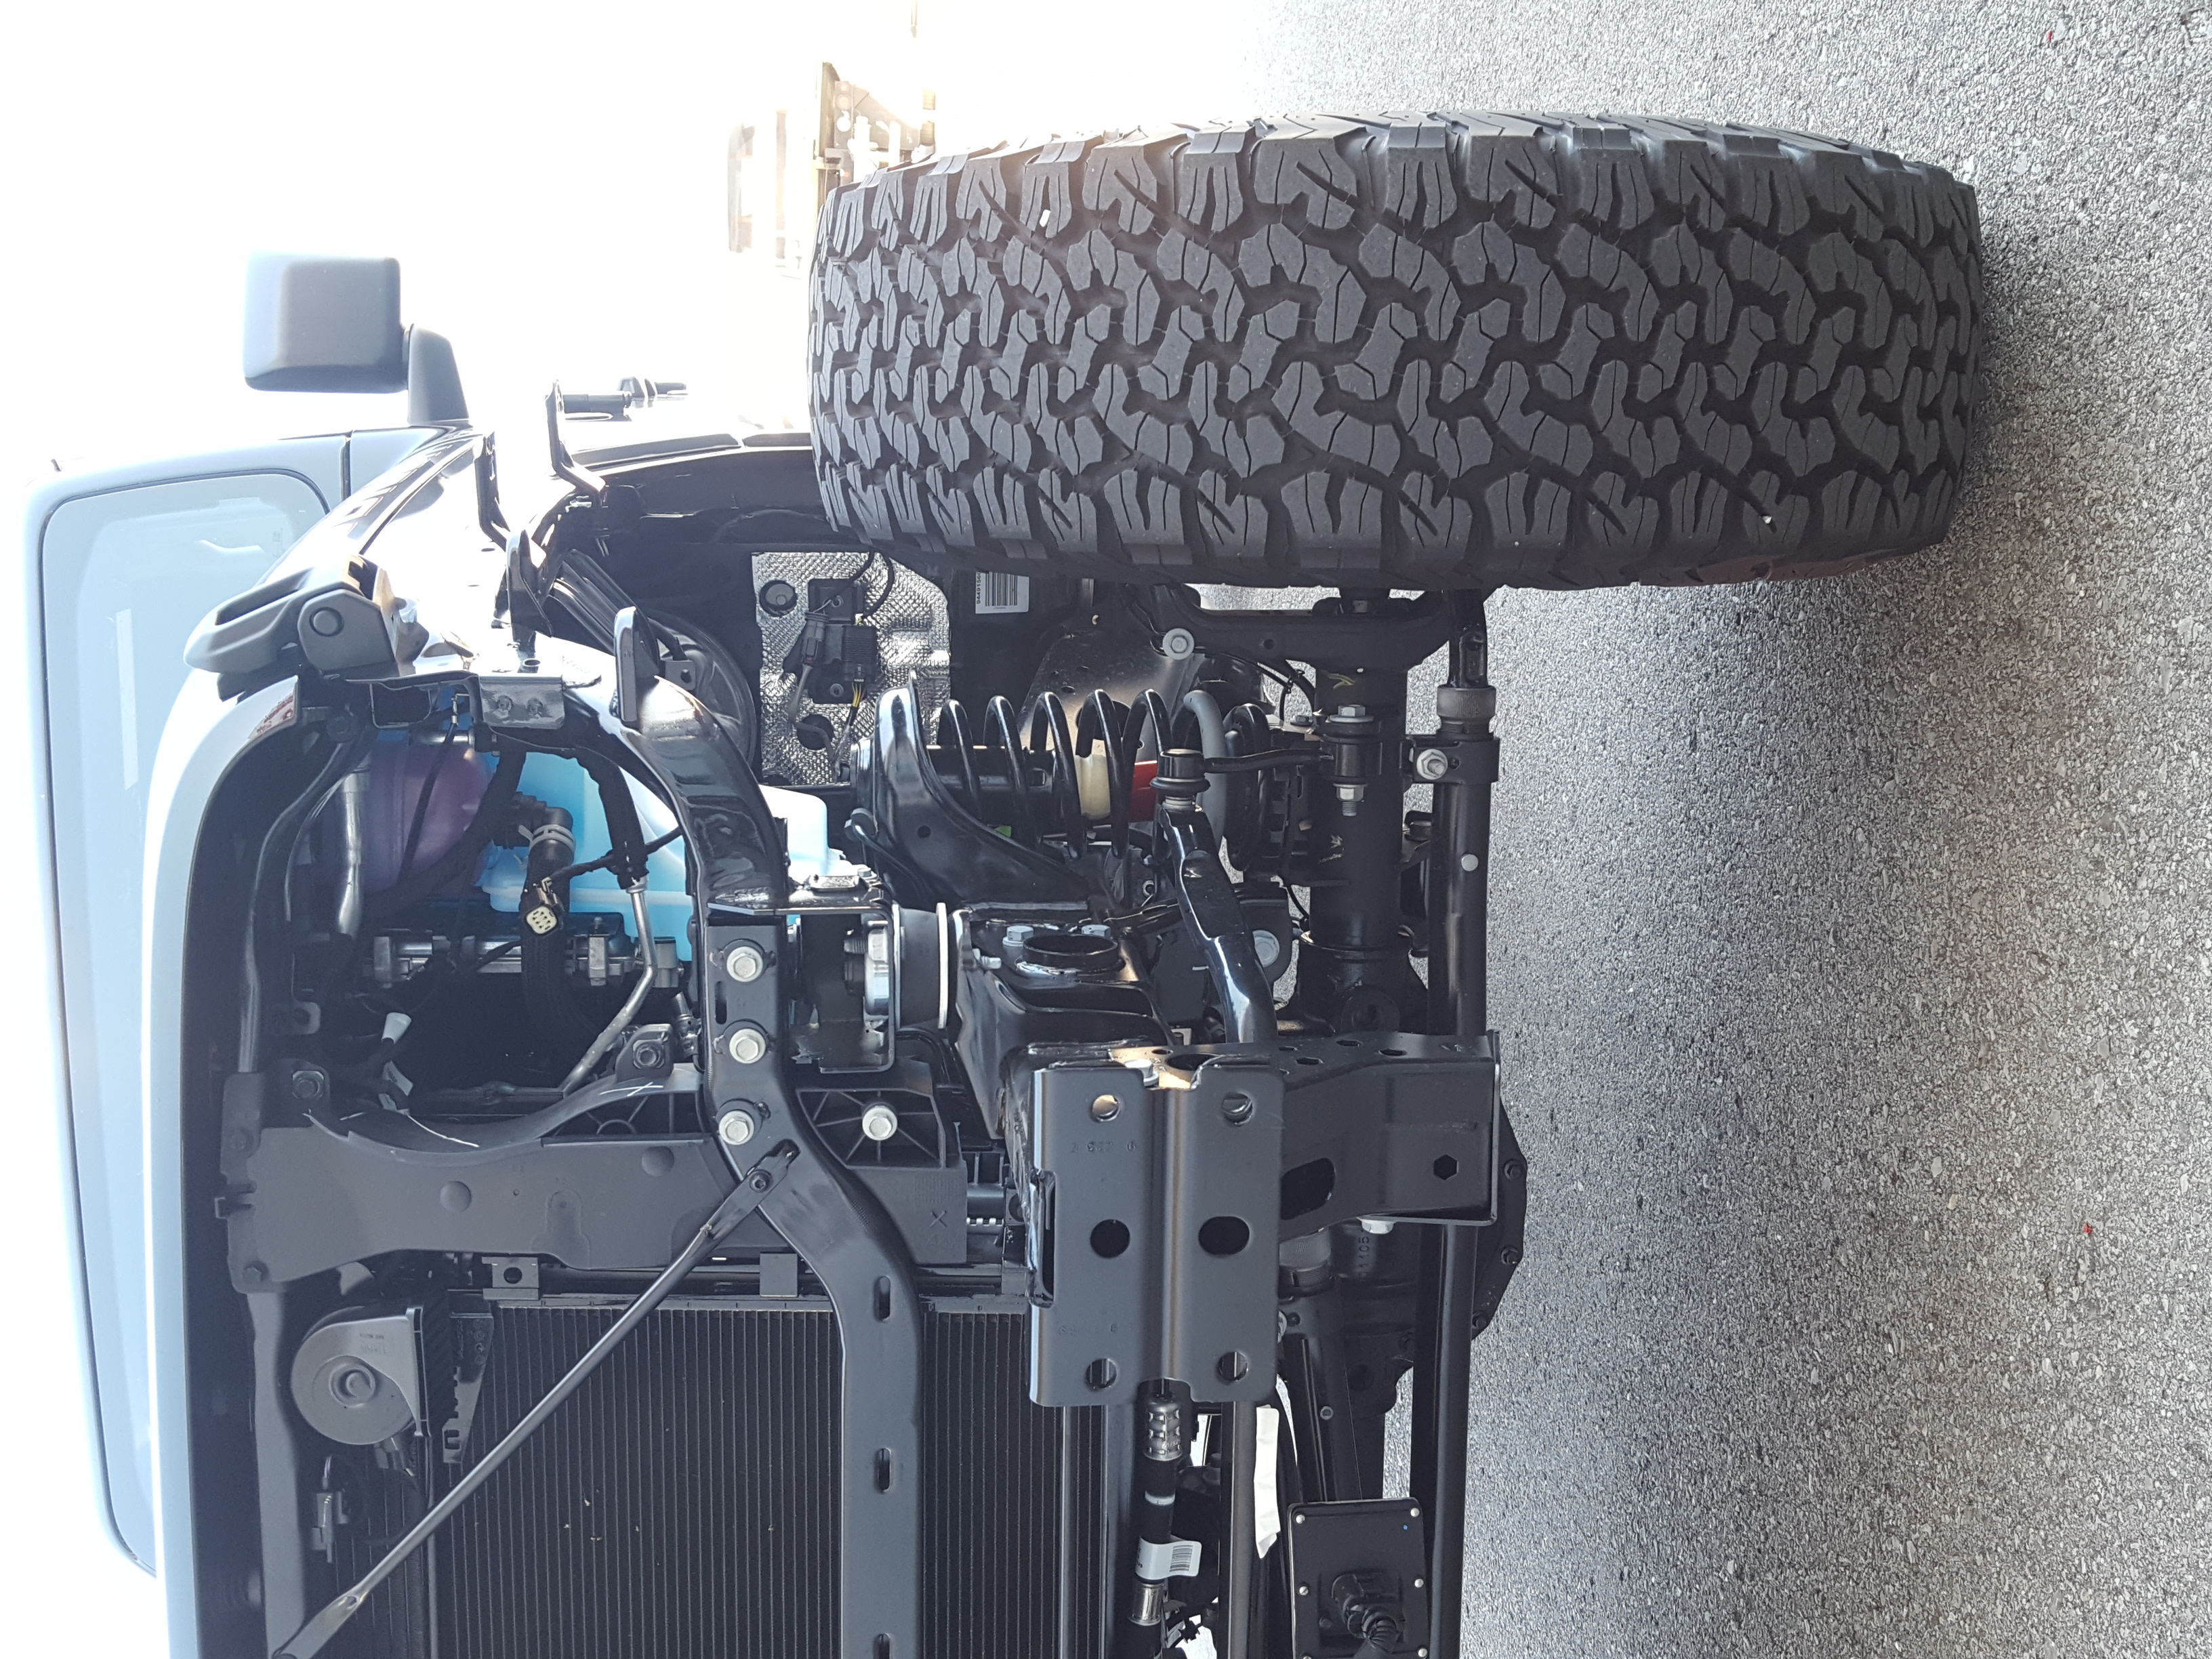
\includegraphics[scale=.1,angle=-90,origin=c]{jeep_01.jpg} 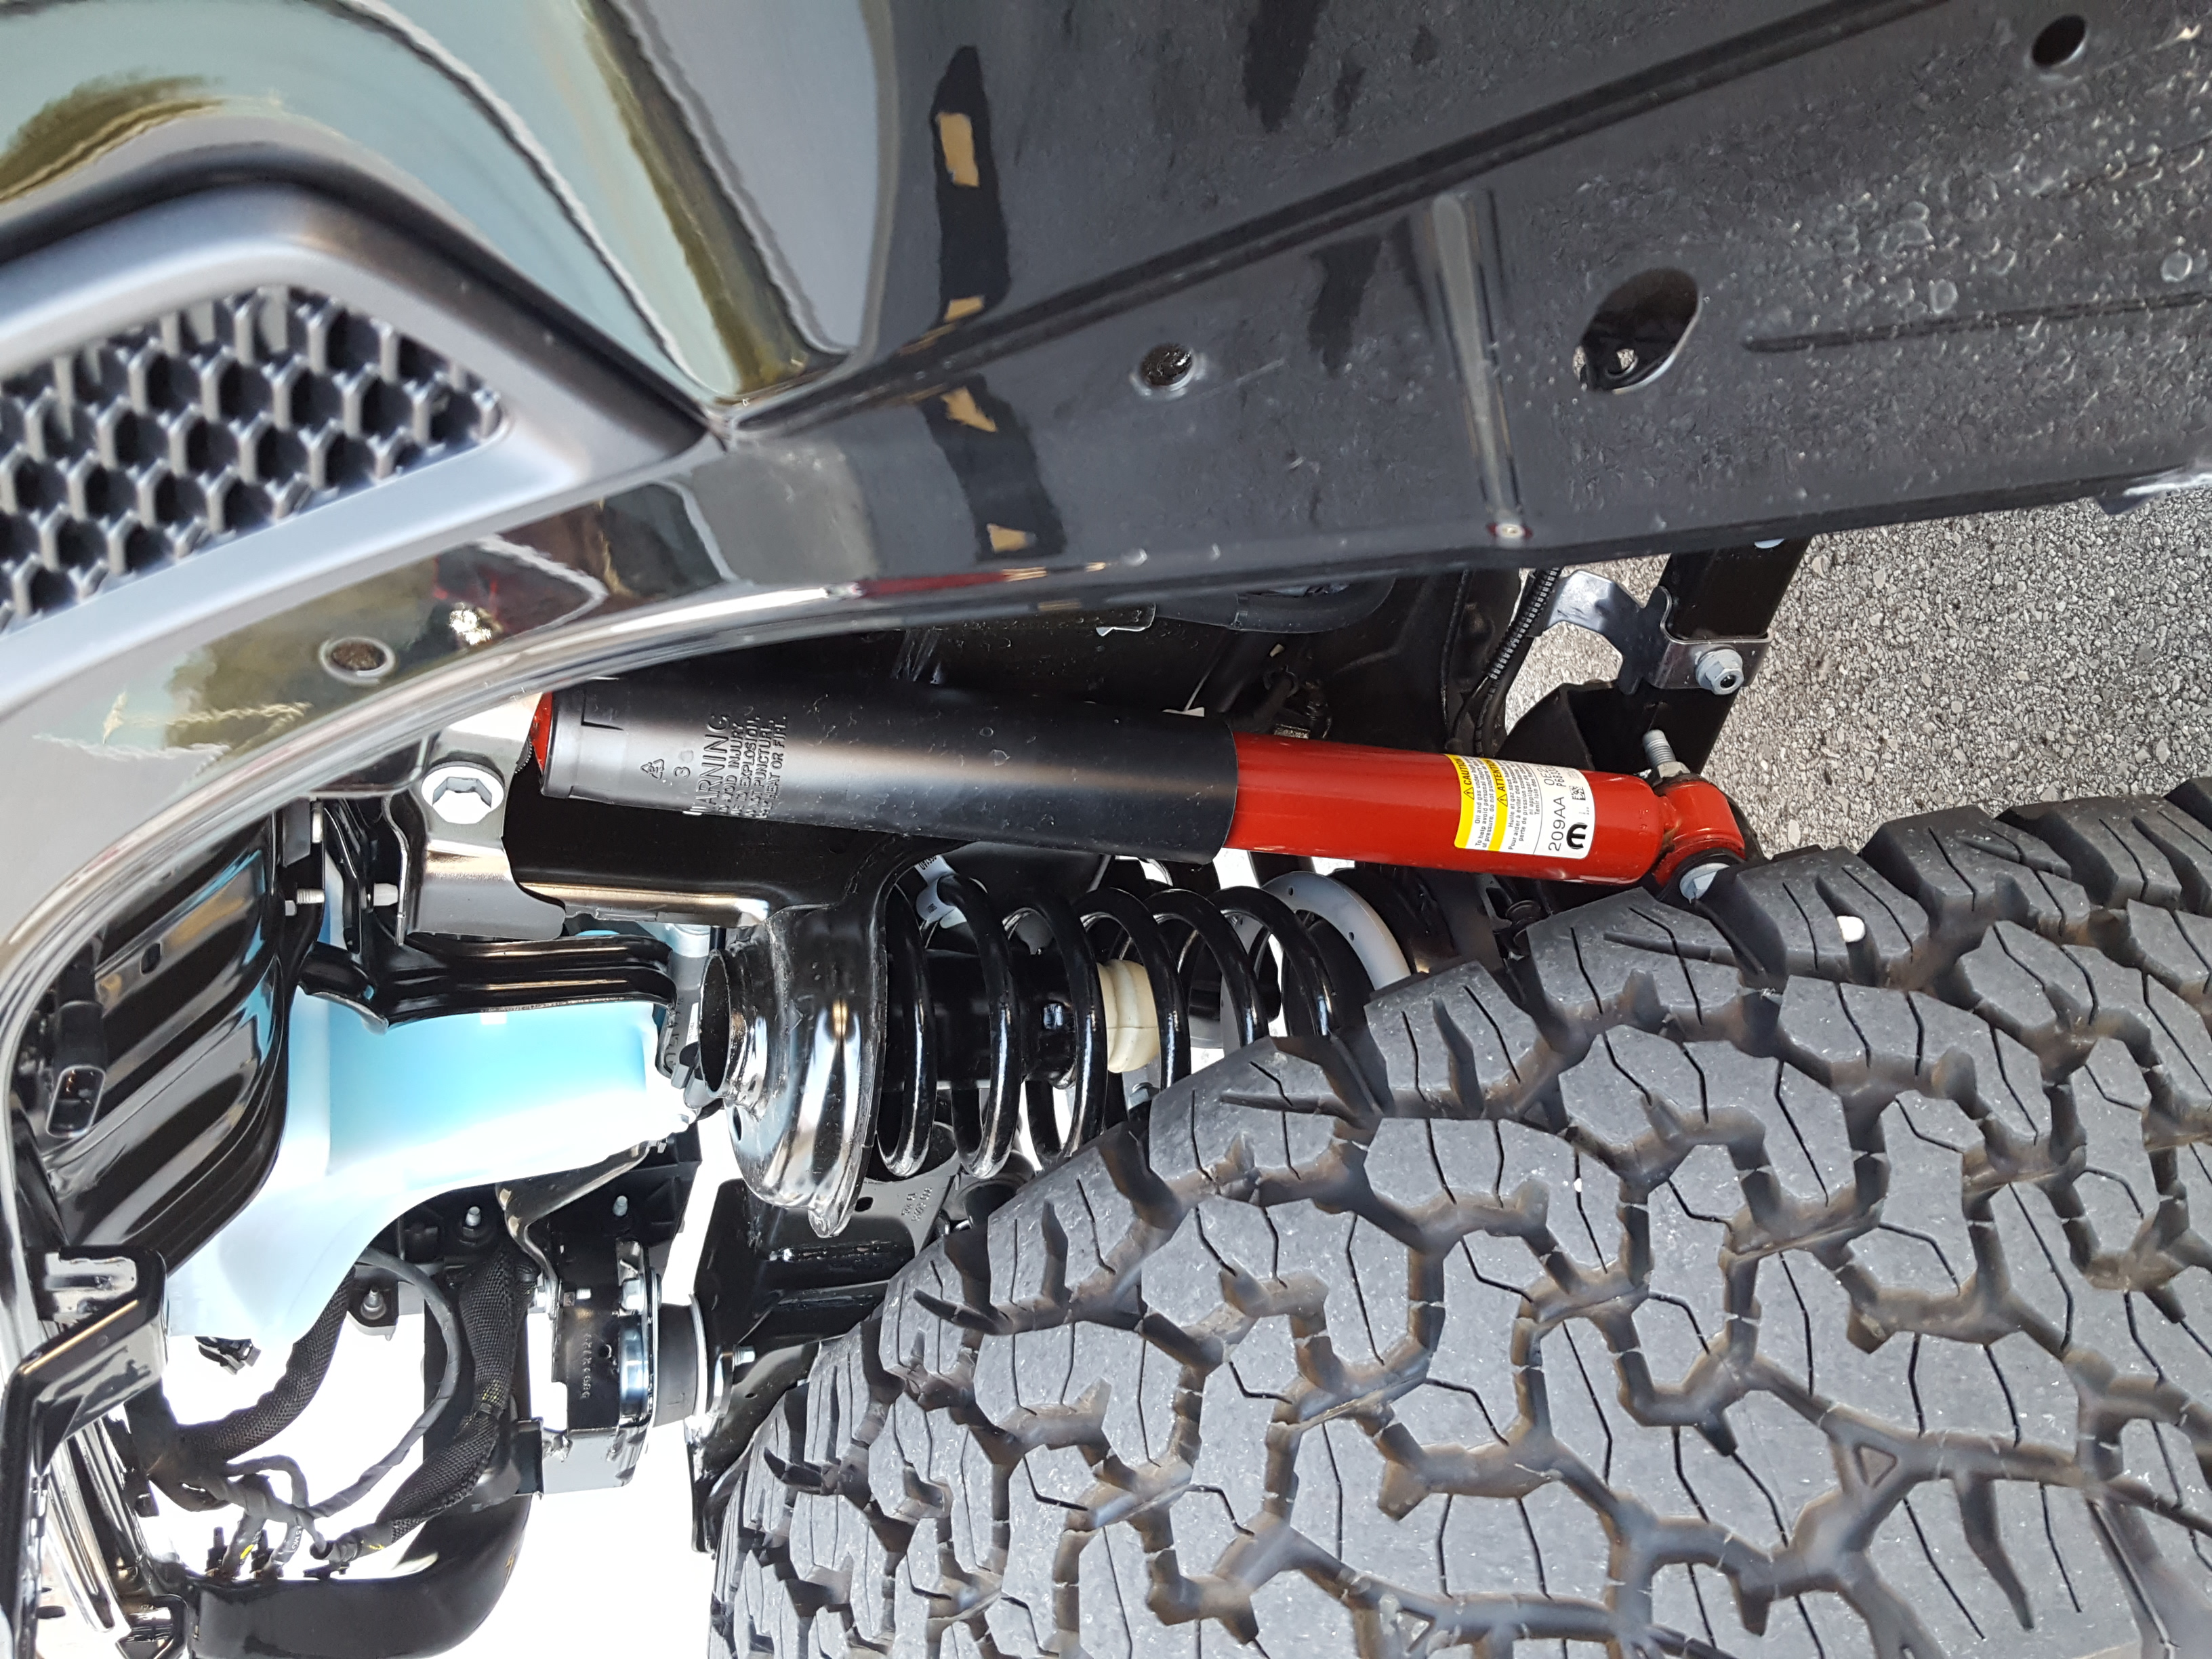
\includegraphics[scale=.1,angle=-90,origin=c]{jeep_02.jpg} \\
%\begin{itemize}
%\item \textbf{ \Large \underline{Problem Statement} -  Derive the \B equations of motion \K using (1) Newton's approach and validate using the (2) Conservation of Energy.}\\
%
%\item \textbf{ \Large \underline{Assumptions} - List the assumptions used in the modeling process.  } 
%
%
%\newpage
%
%\item \textbf{ \Large \underline{Figure(s)} - Draw a \B free body diagram (FBD) \K and/or a sketch of the system. Some problems will require more than one. You need at least one per \B degree of freedom \K.} 
%
%\newpage
%
%\item \textbf{ \Large \underline{Newton's Approach} }\\
%\begin{enumerate}
%\item Draw a Free Body Diagram \vspace{20mm}\\
%\item Determine all \B forces \K acting on the system and their \B directions\K. \vspace{20mm}\\
%\item Write \B Newton's second law \K for the appropriate DOF. \vspace{70mm}\\
%\item Re-write the ODE in the \B standard form \K of a system equation.
%\end{enumerate}
%
%\newpage
%\item \textbf{ \Large \underline{Conservation of Energy Approach} }\\
%\begin{enumerate}
%\item Draw a Free Body Diagram \vspace{20mm}\\
%\item Determine all \B energies \K present in the system and their \B type\K. \vspace{20mm}\\
%\item Write \B Conservation of Energy \K for system. Call this equation 1.\vspace{70mm}\\
%\item Re-write the ODE in the \B standard form \K of a system equation.
%\end{enumerate}
%
%
%\end{itemize}
%
%
%\end{itemize}


	





